\subsubsection{V-Locker}
Die 2019 gegründete Schweizer Firma V-Locker betreibt bisher 4 automatische Systeme zur Lagerung von Fahrrädern.\cite{borkert_interview_2020} Weitere Projekte sind bereits in Planung.\cite{vlockerstandorte}\\
Das Prinzip des Mechanismus ähnelt einem Paternoster: An der Vorderseite können Fahrräder eingelagert werden, innen fahren die Boxen in einem Kreis.\\
Die Investitionssumme des Systems beträgt je nach Ausführung zwischen 5.000€ bis 6.000€ pro Stellplatz.\cite{vlockerpreis} Der Nachteil des Systems liegt an der geringen Größe, es bietet nur Platz für maximal 20 Fahrräder.\\

\begin{figure}[H]
    \centering
    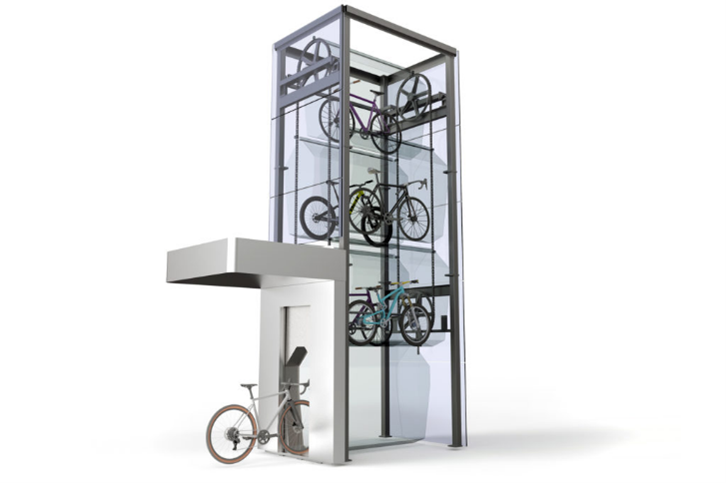
\includegraphics[width=0.5\textwidth]{images/vlocker.png}
    \caption{Funktionsweise vom V-Locker \cite{vlockerbild}}
    \label{fig:vlocker}
\end{figure}
